
\tikzset{every picture/.style={line width=0.75pt}} %set default line width to 0.75pt

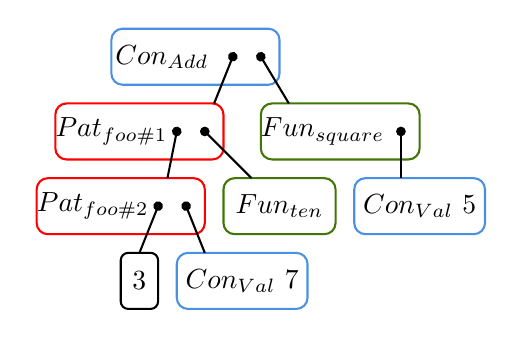
\begin{tikzpicture}[x=0.75pt,y=0.75pt,yscale=-0.9,xscale=0.9]
%uncomment if require: \path (0,440.8571319580078); %set diagram left start at 0, and has height of 440.8571319580078

%Rounded Rect [id:dp48618213158536694]
\draw  [color={rgb, 255:red, 74; green, 144; blue, 226 }  ,draw opacity=1 ] (190,196) .. controls (190,192.69) and (192.69,190) .. (196,190) -- (254,190) .. controls (257.31,190) and (260,192.69) .. (260,196) -- (260,214) .. controls (260,217.31) and (257.31,220) .. (254,220) -- (196,220) .. controls (192.69,220) and (190,217.31) .. (190,214) -- cycle ;

%Rounded Rect [id:dp009025103452140248]
\draw  [color={rgb, 255:red, 74; green, 144; blue, 226 }  ,draw opacity=1 ] (95,236) .. controls (95,232.69) and (97.69,230) .. (101,230) -- (159,230) .. controls (162.31,230) and (165,232.69) .. (165,236) -- (165,254) .. controls (165,257.31) and (162.31,260) .. (159,260) -- (101,260) .. controls (97.69,260) and (95,257.31) .. (95,254) -- cycle ;

%Rounded Rect [id:dp9232511876637792]
\draw  [color={rgb, 255:red, 74; green, 144; blue, 226 }  ,draw opacity=1 ] (60,116) .. controls (60,112.69) and (62.69,110) .. (66,110) -- (144,110) .. controls (147.31,110) and (150,112.69) .. (150,116) -- (150,134) .. controls (150,137.31) and (147.31,140) .. (144,140) -- (66,140) .. controls (62.69,140) and (60,137.31) .. (60,134) -- cycle ;

%Rounded Rect [id:dp10823094494105145]
\draw  [color={rgb, 255:red, 255; green, 0; blue, 0 }  ,draw opacity=1 ] (30,156) .. controls (30,152.69) and (32.69,150) .. (36,150) -- (114,150) .. controls (117.31,150) and (120,152.69) .. (120,156) -- (120,174) .. controls (120,177.31) and (117.31,180) .. (114,180) -- (36,180) .. controls (32.69,180) and (30,177.31) .. (30,174) -- cycle ;

%Rounded Rect [id:dp509725264431323]
\draw  [color={rgb, 255:red, 255; green, 0; blue, 0 }  ,draw opacity=1 ] (20,196) .. controls (20,192.69) and (22.69,190) .. (26,190) -- (104,190) .. controls (107.31,190) and (110,192.69) .. (110,196) -- (110,214) .. controls (110,217.31) and (107.31,220) .. (104,220) -- (26,220) .. controls (22.69,220) and (20,217.31) .. (20,214) -- cycle ;

%Rounded Rect [id:dp3455746100780601]
\draw   (65,234) .. controls (65,231.79) and (66.79,230) .. (69,230) -- (81,230) .. controls (83.21,230) and (85,231.79) .. (85,234) -- (85,256) .. controls (85,258.21) and (83.21,260) .. (81,260) -- (69,260) .. controls (66.79,260) and (65,258.21) .. (65,256) -- cycle ;

%Rounded Rect [id:dp5622973663481885]
\draw  [color={rgb, 255:red, 65; green, 117; blue, 5 }  ,draw opacity=1 ] (140,156) .. controls (140,152.69) and (142.69,150) .. (146,150) -- (219,150) .. controls (222.31,150) and (225,152.69) .. (225,156) -- (225,174) .. controls (225,177.31) and (222.31,180) .. (219,180) -- (146,180) .. controls (142.69,180) and (140,177.31) .. (140,174) -- cycle ;

%Rounded Rect [id:dp33414100410678915]
\draw  [color={rgb, 255:red, 65; green, 117; blue, 5 }  ,draw opacity=1 ] (120,196) .. controls (120,192.69) and (122.69,190) .. (126,190) -- (174,190) .. controls (177.31,190) and (180,192.69) .. (180,196) -- (180,214) .. controls (180,217.31) and (177.31,220) .. (174,220) -- (126,220) .. controls (122.69,220) and (120,217.31) .. (120,214) -- cycle ;

%Straight Lines [id:da7735002123972574]
\draw    (140,125) -- (155,150) ;

\draw [shift={(140,125)}, rotate = 59.04] [color={rgb, 255:red, 0; green, 0; blue, 0 }  ][fill={rgb, 255:red, 0; green, 0; blue, 0 }  ][line width=0.75]      (0, 0) circle [x radius= 2, y radius= 2]   ;
%Straight Lines [id:da19830589256441322]
\draw    (125,125) -- (115,150) ;

\draw [shift={(125,125)}, rotate = 111.8] [color={rgb, 255:red, 0; green, 0; blue, 0 }  ][fill={rgb, 255:red, 0; green, 0; blue, 0 }  ][line width=0.75]      (0, 0) circle [x radius= 2, y radius= 2]   ;
%Straight Lines [id:da7234273703208924]
\draw    (95,165) -- (90,190) ;

\draw [shift={(95,165)}, rotate = 101.31] [color={rgb, 255:red, 0; green, 0; blue, 0 }  ][fill={rgb, 255:red, 0; green, 0; blue, 0 }  ][line width=0.75]      (0, 0) circle [x radius= 2, y radius= 2]   ;
%Straight Lines [id:da39520289035501]
\draw    (110,165) -- (135,190) ;

\draw [shift={(110,165)}, rotate = 45] [color={rgb, 255:red, 0; green, 0; blue, 0 }  ][fill={rgb, 255:red, 0; green, 0; blue, 0 }  ][line width=0.75]      (0, 0) circle [x radius= 2, y radius= 2]   ;
%Straight Lines [id:da4431461097782077]
\draw    (215,165) -- (215,190) ;

\draw [shift={(215,165)}, rotate = 90] [color={rgb, 255:red, 0; green, 0; blue, 0 }  ][fill={rgb, 255:red, 0; green, 0; blue, 0 }  ][line width=0.75]      (0, 0) circle [x radius= 2, y radius= 2]   ;
%Straight Lines [id:da8121818084178258]
\draw    (85,205) -- (75,230) ;

\draw [shift={(85,205)}, rotate = 111.8] [color={rgb, 255:red, 0; green, 0; blue, 0 }  ][fill={rgb, 255:red, 0; green, 0; blue, 0 }  ][line width=0.75]      (0, 0) circle [x radius= 2, y radius= 2]   ;
%Straight Lines [id:da8679389234287274]
\draw    (100,205) -- (110,230) ;

\draw [shift={(100,205)}, rotate = 68.2] [color={rgb, 255:red, 0; green, 0; blue, 0 }  ][fill={rgb, 255:red, 0; green, 0; blue, 0 }  ][line width=0.75]      (0, 0) circle [x radius= 2, y radius= 2]   ;

% Text Node
\draw (225,205) node   {$Con_{Val} \ 5$};
% Text Node
\draw (130,245) node   {$Con_{Val} \ 7$};
% Text Node
\draw (87,125) node   {$Con_{Add}$};
% Text Node
\draw (60,165) node   {$Pat_{foo\#1}$};
% Text Node
\draw (50,205) node   {$Pat_{foo\#2}$};
% Text Node
\draw (75,245) node   {$3$};
% Text Node
\draw (173.05,165) node   {$Fun_{square}$};
% Text Node
\draw (150,205) node   {$Fun_{ten}$};

\end{tikzpicture}
